\documentclass[11pt,twocolumn]{witseiepaper}
\RequirePackage{ifpdf}
\usepackage{amsmath}
\usepackage{amssymb}
\usepackage{KJN}
\usepackage{pdfpages}
\renewcommand*{\bibfont}{\small}

\ifpdf
\pdfinfo{
	/Title (Research Proposal)
	/Author (Alice Yang (597609))
}
\fi

\begin{document}
	\title{Masters Research Proposal - Dimensionality reduction techniques in pattern recognition with different types of x-ray images }
	
	\author{Alice Yang (597609) \thanks{School of Electrical and Information Engineering, University of the Witwatersrand, Private Bag 3, 2050, Johannesburg, South Africa} }
	
	\abstract{This paper proposes a research in determining the optimal dimensionality reduction technique for a two-step system for bone fracture detection. The two-step system consists of a dimensionality reduction technique and a neural network component. In addition, an image pre-processing module is to be implemented. The module produces 26 different processed images from the original image. Furthermore, the pre-processing module extracts three features, namely gradient, lines and contours. The dimensionality reduction techniques proposed for comparison are Principal Component Analysis (PCA), Kernel Principal Component Analysis (KPCA) and Maximum Variance Unfolding (MVU). The proposed training technique for the neural network is back-propagation. To determine the optimal dimensionality reduction technique, the performance for each technique is compared. The performance is based on high detection accuracy, low error rate and execution time. Further investigation will be conducted to extend the two-step system for the detection of Tuberculosis disease (TB) as well as exending it to the manufacturing field. In the manufacturing field, the system can be utilized to detect fractures or inconsistancies within the manufactured components.}
	
	\keywords{Dimensionality Reduction Techniques, Back-Propagation Neural Network, Bone Fracture Detection, Two-Step System, Principal Component Analysis, Kernel Principal Component Analysis, Maximum Variance Unfolding}
	\maketitle
	\thispagestyle{empty}\pagestyle{empty}
	
	\section{Introduction}
	In the medical field there is an emphasis on the importance of medical diagnosis. In critical cases, an inaccurate diagnosis of a symptom can cost a patient's life. Most diagnoses are performed by trained medical doctors, however they are prone to making mistakes which can be influenced by external factors such as fatigue and lack of training in the particular field. Automation of medical diagnosis was introduced in the early 1970s \cite{Ramesh2004}. There are many algorithms available designed with the aim of diagnosing patients. The basic algorithm consists of "if... then..." statements. Although the algorithm is simple, the list of conditions in the medical field are endless and as a result the execution time to diagnosis a patient's symptoms is not realistic. 
	
	This proposal discusses the procedures taken to conduct research in discovering the best dimensionality reduction technique for a two-step system for detecting the presence of a bone fracture. The two-step system is defined as having a dimensionality reduction and neural network module. The purpose of introducing dimensionality reduction to the system is to compress the input data. The input data into the system are raw X-ray images. Raw X-ray images are large data files, which can make it difficult to train the neural network.
	
	In addition to detecting bone fractures, further investigations will be conducted to extend the system to detect the presence of Tuberculosis disease (TB). The system is further extended to the manufacturing field to detect fractures within axle components. Section \ref{sc: Background} and \ref{sc: Literature Review} presents the Background and Literature Review respectively. Section \ref{sc: Proposed Methodology} shows the Proposed Methodology to conduct the research. Section \ref{sc: Time Management and Milestones} illustrates the Time Management and Milestones that need to be achieved for the research and Section \ref{sc: Conclusion} concludes the proposal. 
	
	\section{Literature Review}
	\label{sc: Literature Review}
	The automation of bone fracture detection is becoming increasingly popular. This is mainly due to the difficulty of applying manual analysis to the increasing volume of image data. The difficulty lies in the lack of human expertise, poor image quality and time. The solution to this problem has been explored by various biomedical and engineering professionals. 
	
	A technique that outlines the fractured bones in an X-ray image of a patient's arm within casting material is presented by \cite{Jia_Jiang2006}. The technique divides the image into segments, since the casting material causes a low contrast and high noise ratio within the X-ray image. To eliminate the noise, a geodesic active contour model with global coefficients is applied to the segments of bone region. The global constraint for the model is predefined by the prior shape collected. Feedback for each iteration is provided by a maximum-likelihood function. The experimental results obtained by the authors indicated that the technique produces outlines of the fractured bones on the low contrast X-ray images in a robust and accurate manner.
	
	Liang et al. proposed a technique which makes use of mathematical morphology to identify tibia bone fractures \cite{Liang_Pan_Huang_Fan_2010}. The technique applies segmentation to the x-ray images by dynamically dividing it into several intervals to determine the smallest intervals with the target. The technique makes use of the Otsu method to automatically threshold the small regions. A statistical method is employed for examining the segments to ensure that accuracy is achieved and to prevent over- or under-segmentation. The segments of the image are adjusted accordingly to the results obtained from each iteration. The iterations end when the test result conforms to predefined stopping conditions. The segmentation process is then followed by mathematical morphology, in which the target border as well as boundary fractures are extracted. The precise location of fractures is detected by superposing the target border image to extracted skeleton.
	
	An automated fracture detection system for long bones has been developed by the authors of \cite{Donnelley2005}. The system first extracts the edges of the x-ray image using a non-linear anisotropic diffusion method. The diffusion method operates by smoothing the image without discarding crucial information regarding the boundary locations. The second step is to determine parameters for the straight lines that best represent the edges of the long bones. This is done modifying the Hough transform which has an automatic peak detection. To highlight the abnormal regions which includes fractures, the magnitude and direction of the gradient is determined by making use of the calculated parameters.
	
	In \cite{Syiam_Aziem_Soliman2004}, an adaptive interface agent (AdAgen) that incorporates trained agents using neural network is proposed. The neural network is used to build the software interface agent for the detection of fractures in long bones. A semi-intelligent system is provided by the software agent. The results obtained from the simulations indicates that the incorporated agents assists with the performance of the automated fracture detection in leg radiography.
	
	The general approach to classifying the presence of bone fracture involves mapping the data to one of several predefined classes. However, there are challenges presented 
	in the classification technique which are due to information overload, size and dimension of the data \cite{Mahendran2011}. According to \cite{Mahendran2011}, a classification technique is defined as a systematic approach of processing data input by constructing classification models. Examples of classification techniques includes Decision Tree Classifiers, Rule-Based Classifiers, Neural Networks, Support Vector Machines and Na\"{i}ve Bayes Classifiers.
	
	There are various standard classifiers implemented for automating the detection of bone fractures using x-ray images. \cite{Mahendran2012} describes a study done to test the performance of single and combination classifiers. The classifiers used in the study are Back-Propagation Neural Network (BPNN), Support Vector Machine (SVM) and Na\"{i}ve Bayes (NB) classifiers. Contrast, Homogeneity, Energy, Entropy, Mean, Variance, Standard Deviation Correlation, Gabor orientation (GO), Markov Random Field (MRF) and intensity gradient direction (IGD) are features exacted for testing each classifier. The metrics used to evaluate the performance of each classifier are sensitivity, specificity, positive predictive value, negative predictive value, accuracy and execution time. The authors discovered that fusion classifiers enhances the detection capacity. Furthermore, the results indicated that the combination of SVM and BPNN obtained the best performance.
	
	\cite{Mahendran_Enhanced} proposes a four-step system that makes use of fusion-classification techniques to automated the detection of bone fracture specifically for leg bones (Tibia). The four-steps are preprocessing, segmentation, feature extraction and bone detection. The three classifiers during the fusion classification are Feed Forward Back-Propagation Neural Network (BPNN), Support Vector Machine (SVM) and Na\"{i}ve Bayes Classifiers (NB). Through experimentation, the authors stated that the proposed four-step system showed significant improvement in terms of detection rate and speed of classification.
	
	In \cite{ComputerAidedBoneFractureDetection}, the authors proposed a system based on Artificial Neural Network (ANN) for the detection of bone fractures. The system is designed to accept X-ray images as its input. The images are then enhanced using pre-processing techniques. The ANN module is trained using the enhanced x-ray images. "\textit{True Detection Rate}" and "\textit{False Detection Rate}" are used to evaluate the performance of the system. The results that authors obtained for the proposed system indicated that the system had a 89\% success rate.
	
	\cite{lim2004detection} describes an approach for automating the detection of bone fractures in the femur and radius. The system consists of a combinational approach. The first step of the system is to pre-process the input, by extracting features, namely Gabor texture, Markov Random Field texture and intensity gradient. The classifiers implemented for testing are Bayesian classifier and Support Vector Machine (SVM). From experimental results, the combined approach improved the detection rate of bone fractures as well as the classification accuracy compared to a single classification approach.
	
	\cite{JoshuaCongfuHe2007} presents a fracture detection technique which partitions the problem into smaller sub-problems. The sub-problems lie within the SVM kernel space. The training process trains multiple SVMs, such that each sub-problem can be solved by a specialized SVM, therefore forming a hierarchy of SVMs. The experimental results obtained indicates that the hierarchy of SVMs performs better than a single SVM. Furthermore, the performance showed that it enhanced the accuracy and reliability of SVMs.
	
	\cite{multiple_classification} presents a multiple classification system which detects fractures in long bones (Tibia). The features used for the system are texture and shape. The system makes use of three different classifiers, namely Back Propagation Neural Network, K-Nearest Neighbour and Support Vector Machine. Each classifier is trained with different sets of data. Fusion selection is adopted as the voting scheme used for decision making. The decisions made by the system is binary. It indicates the whether there is a fracture present or absent.
	
	\cite{Li_Liang2016} presents a convolutional neural network (CNN) model that automatically detect lumbar vertebrae in C-arm and X-ray images. The training of data is done by making use of Disaster Risk Reduction (DRR). The computational complexity is reduced by automatic segmentation of Region of Interest (ROI). A feature fusion deep learning (FFDL) model is included to combine the two features of lumbar vertebra X-ray images. This makes use of sobel kernel and Gabor kernel to extract the features namely, contour and texture. From the experiments, the authors found that the proposed model performed more accurately in abnormal cases with pathologies and surgical implants. 
	
	The authors of \cite{Pune2016} proposed a system that extracts features and classify lung diseases using an artificial neural network. The lung diseases includes Tuberculosis (TB), lung cancer and pneumonia. The detection of the lung boundaries is done by pre-processing the image. The pre-processing technique is based on intensity and discontinuity methods. The features extracted are statistical and geometrical features. For image classification, the system makes use of feed forward and back propagation neural network to detect lung diseases. 
	
	Outside of the medical field, there are various studies which combine both supervised and unsupervised learning. The authors of \cite{neagoe_new_2014} proposed a neural network based approach for automatic annotation of remote sensing imagery. The proposed model consists of Self-Organizing Map (SOM) as its unsupervised pattern recognition along with the supervised classifier of Concurrent (CSOM). The performance of the model is compared to classical statistical techniques which made use of Latent Dirichlet Allocation(LDA) and K-Means. The experimental results indicated that the proposed model was effective.
	
	The paper, \cite{Baqqar2012} focuses on developing a monitoring system for gearbox production. The system is based on operating parameters. These parameters are available in the machine control process. By making use of the machine control process, other additional measurements namely, vibration and acoustics can be discarded. The system proposed examines the data model using General Regression Neural Network (GRNN) to utilize the parameters. The GRNN captures the non-linear connections between the electrical current for the driving motor and the control parameters. The detection of abnormal gearbox conditions are done by comparing the measured and the predicted values. An abnormal gearbox condition is defined by the different gear tooth breakages which is based on a setup threshold in the system.
	
	\cite{kottaimalai_eeg_2013} designed a system in which it consists of a Principal Component Analysis(PCA) and a Neural Network module for the classification of EEG Signals. The authors compared the performance of the classification to a single neural network module. The final outcome from the experimentation is that the performance of the classification of the Principal Component Analysis with Neural Network system is better than Neural Network alone.  
	
	\section{Background}
	\label{sc: Background}
	The review done by Mahendran et al. for the automation of bone fracture detection indicated that there are various techniques in pattern recognition that comes in the form of unsupervised, reinforcement and supervised \cite{Mahendran2011}. The challenge found in classification is that there is an information overload and size and dimension are a concern. The problem with information overload is that it becomes computationally expensive to find crucial information needed for the classification. The size and dimension of the information is a concern because large quantities of data increases the number of dimensionalities. A high number of dimensions presents a challenge in the classification process and in turn may require more computational resources.
	
	\subsection{Curse of Dimensionality}
	The main problem affecting the performance in classification is the curse of dimensionality. The curse of dimensionality arises from the sparsity of high dimensional spaces, in which an absurd amount of training data is needed in order to get low variance  estimators \cite{intrator_feature_1992}.
	
	Feature extraction with supervised learning algorithms may seem more desirable when compared to unsupervised learning algorithms since supervised learning algorithms have more information about the problem and features. However, unsupervised methods do not suffer from the curse of dimensionality to the same extent as supervised learning. This is because it makes use of local measures to optimally estimate a single dimensional projection  function\cite{intrator_feature_1992}.
	
	\subsection{Dimensionality Reduction}
	The collection of digital data has increased drastically over the past decade, which led to high dimensionality datasets. The increase in dimensionality affected the performance of data processing algorithms, also known as the curse of dimensionality \cite{Center2002}. Dimensionality reduction decreases the number of random variables found within the considered dataset. This process can be divided into two stages, namely Feature Selection and Feature Extraction. Both these stages are crucial for automating bone fracture detection. There are two types of dimensionality techniques, convex and concave. 
	
	Convex techniques optimize objective functions that do not contain any local optima, indicating a convex solution space \cite{Boyd2010}. The objective function is usually in a generalized Rayleigh quotient, which can be expressed in the following form: 
	\begin{equation}
	\phi(\textbf{Y}) = \frac{\textbf{Y}^{T}\textbf{AY}}{\textbf{Y}^{T}\textbf{BY}}
	\label{eq: general objective function}
	\end{equation}
	The function expressed in the form of \eqref{eq: general objective function} can be easily optimized by solving a generalized eigenproblem. Convex dimensionality reduction techniques can be subdivided into techniques that perform eigendecomposition on full and sparse matrix. The following section focuses on the eigendecomposition of full matrices. 
	
	\subsubsection{Principal Component Analysis and Classical Scaling}
	Principal Component Analysis (PCA) is a linear technique that performs dimensionality reduction through the process of embedding the data into a linear subspace of low-dimensionality. The low-dimensional representation of the data describes the variance of the data \cite{Jolliffe2016}. During the construction of the low-dimensional representation, PCA does not discard information, instead it creates new characteristics to represent the original characteristics. This is done by searching for characteristics that show the largest variation. Additionally, PCA searches for characteristics that allows for the reconstruction of the original characteristics from the new characteristics. According to \cite{van2009dimensionality}, maximizing the variance will result in minimizing the error. Hence, the construction of the low-dimensional representation is obtained by determining mapping function,  \textbf{M}, which maximizes the cost function. The cost function is expressed in \eqref{eq: scaling cost function}.
	\begin{equation}
	\phi(\textbf{Y}) = \sum_{ij}(d_{ij}^{2} - ||\textbf{y}_i - \textbf{y}_j||^2)
	\label{eq: scaling cost function}
	\end{equation}
	where 
	
	$||\textbf{y}_i - \textbf{y}_j ||^{2}$ = squared Euclidean distance between low-dimensional datapoints $\textbf{y}_i$ and $\textbf{y}_j$
	
	Eigenvectors and eigenvalues are solved using the eigenproblem expressed in \eqref{eq: eigenproblem}. Eigenvectors and eigenvalues are crucial in PCA since eigenvectors assist with determining the correlation between the data points whilst eigenvalues, $\lambda$ dictates the weighted average of the variance for any projection.
	\begin{equation}
	cov(\textbf{X})\textbf{M} = \lambda\textbf{M}
	\label{eq: eigenproblem}
	\end{equation}
	The disadvantage with PCA is that the size of the covariance matrix is dependent on the dimensionality of the original dataset. This means that the size of the covariance matrix is proportional to the number of dimensionalities presented by the dataset, which can result in the inability to compute eigenvectors for very high-dimensional datasets \cite{van2009dimensionality}.
	
	Classical Scaling is an identical technique to PCA, however Classical Scaling searches for the linear mapping  function, \textbf{M}, that minimizes the cost function that is expressed in \eqref{eq: scaling cost function}. Furthermore, the low-dimensional representation is of the Gram Matrix in which the double-centering pairwise squared Euclidean distance matrix entries are obtained using \eqref{gram_enteries}.
	\begin{equation}
	k_{ij} = -\frac{1}{2}(d_{ij}^{2}-\frac{1}{n}\sum_{l}d_{il}^{2} - \frac{1}{n}\sum_{l}d_{jl}^{2} + \frac{1}{n^2}\sum_{lm}d_{lm}^{2})
	\label{gram_enteries}
	\end{equation}
	where 

	$d_{ij}^2, d_{il}^2, d_{jl}^2, d_{lm}^2$ are Squared pairwise Euclidean distances.
	
	The disadvantage for both PCA and Classical Scaling is the cost function in \eqref{eq: scaling cost function} focuses on retaining large pairwise distances, $d_{ij}^2$, whereas retaining the small pairwise distance can be important for minimizing error.
	
	\subsubsection{Isomap}
	Unlike PCA and Classical Scaling where the aim of the techniques is to retain the pairwise Euclidean distances, the Isomap technique attempts to preserve the pairwise geodesic distances between data points \cite{Zhang2012}. This means that the geodesic distance between $x_i$ and $x_j$ imitates as much of the Euclidean between the low-dimensional representation $y_i$ and $y_j$ as possible. The low-dimensional representation $y_i$ and $y_j$ are computed using the classical scaling technique, which results in a pairwise geodesic distance matrix. The drawback of the Isomap technique is that it constructs erroneous connections in the neighbourhood graph, G, which can affect the performance of the Isomap. The neighbourhood graph is a method which constructs a mapping scheme for non-linear dimensional reduction techniques \cite{Aeini2014}.
	
	\subsubsection{Kernel PCA}
	Kernel Principal Component Analysis (KPCA) is a technique that makes use of kernel functions to map data into high dimensional space. The space is manipulated using linear PCA \cite{Cui2012}. KPCA makes use of a mapping function which computes the kernel matrix, $K$ of data points $x_i$ and $x_j$. The entries for the kernel matrix are defined by \eqref{eq: kernel matrix enteries}.
	\begin{equation}
		k_{ij} = K(x_i, x_j)
		\label{eq: kernel matrix enteries}
	\end{equation}
	where
	\begin{align*}
		K &= \text{kernel function}\\
		x_i \text{ and } x_j &= \text{input data points}
	\end{align*}
	The features defined by the kernel function have a zero-mean. Additionally, the eigenvectors of the covariance matrix, $\textbf{a}_i$, which is expressed in \eqref{eq: kernel covariance matrix} can be computed, since the eigenvectors of the kernel matrix are related. 
	\begin{equation}
		\textbf{a}_i = \frac{1}{\sqrt{\lambda_i}} \textbf{v}_i
		\label{eq: kernel covariance matrix}
	\end{equation}
	where
	\begin{align*}
		\textbf{v}_i &= \text{eigenvector} \\
		\lambda_i &= \text{eigenvalue}\\
	\end{align*}
	The low-dimensional representation is obtained by the projection given by \eqref{eq: kernel low-dimensional}.
	\begin{equation}
		\textbf{y}_i = \left\{ \sum_{j = 1}^{n}a_1^{(1)}K(\textbf{X}_j, \textbf{X}_i), ... , \sum_{j = 1}^{n}a_d^{(j)}K(\textbf{X}_j, \textbf{X}_i) \right\}
		\label{eq: kernel low-dimensional}
	\end{equation}
	where
	\begin{align*}
		a_1^{(j)} &= \text{jth value in vector }\textbf{a}_1
	\end{align*}
	A disadvantage with KPCA is that the size of the kernel matrix is proportional to the square number of instances in the dataset. However despite the obvious disadvantages, KPCA is applied to facial recognition, speech recognition and novelty detection \cite{van2009dimensionality}.
	
	\subsubsection{Maximum Variance Unfolding}
	Maximum Variance Unfolding (MVU) is a technique that aims to preserve as much of the distances and angles between nearby points as possible by studying the kernel matrix. As a result it forms a neighbourhood graph, $G$ \cite{Jiang2011}. A quadratic equation is formulated for the "unfolding" transformation. The "unfolding" transformation is where MVU maximizes the sum of the squared Euclidean distances between all the data points whilst preserving the distances within neighbouring points. This can be described in \eqref{eq: optimization problem}.
	\begin{equation}
		\text{Max } \sum_{ij}||\textbf{y}_i - \textbf{y}_j||^{2}
		\label{eq: optimization problem}
	\end{equation}
	\begin{align*}
		\text{Subject to:}
		\begin{cases}
			(1)||\textbf{y}_i - \textbf{y}_j||^{2} = ||\textbf{x}_i - \textbf{x}_j||^{2} , \eta_{ij} = 1 \\
			(2)\sum_{i}\textbf{y}_i = 0
		\end{cases}
	\end{align*}
	MVU reformulates the optimization as semi-definite programming (SDP) over matrix $\textbf{K}$ by defining the inner product of $\textbf{K}_{ij} = \textbf{y}_i \cdot \textbf{y}_j$. Thus the SDP can be written as follows: 
	\newline
	Maximize trace(\textbf{K}) subjected to:
	\begin{equation}
		\begin{cases}
			(1) \textbf{K} \geq 0 \\
			(2) \sum_{ij} \textbf{K}_{ij} = 0 \\
			(3) \textbf{K}_{ii} - 2\textbf{K}_{ij} + \textbf{K}_{jj} = ||\textbf{x}_i - \textbf{x}_j||^{2}, \eta_{ij} = 1
		\end{cases}
	\end{equation} 
	From the first condition $\textbf{K} \geq 0$, it indicates that matrix $\textbf{K}$ is required to be positive semi-definite, since SDP is convex. Thus the low-dimensional representation is obtained by solving the SDP. The main weakness found in MVU is the addition of constraints during optimization, which can result in unsuccessful unfolding of the manifold. Despite this main weakness it is applied to sensor location and DNA micro-array data analysis \cite{van2009dimensionality}.
	
	\subsubsection{Diffusion Maps}
	Diffusion Maps (DM) is a technique based on defining a Markov Random Walk graph \cite{COIFMAN20065}. A Markov Random Walk is a description of a random process that consists of the successful random steps applied to a mathematical space. The measurement for the proximity of the data points is attained by performing the random walk for a number of iterations. Through the number of iterations, the diffusion distances are obtained which are used for the representation of the data in the lower dimension. The purpose of the diffusion distance is to integrate over all the paths presented in the graph. For the construction of the diffusion maps graph, the weights of the edges are computed using the Gaussian kernel function. The entries to form matrix \textbf{W} is expressed in \eqref{eq: W entries}.
	\begin{equation}
		w_{ij} = e^{-\frac{||\textbf{x}_i - \textbf{x}_j||^2}{2\sigma^2}}
		\label{eq: W entries}
	\end{equation}
	where
	\begin{align*}
		\sigma &= \text{variance of the Gaussian}\\
		x_i, x_j &= \text{input data points}
	\end{align*}
	The normalization of matrix, \textbf{W} is necessary to defining the forward transition probability matrix of dynamic process. The normalized matrix, \textbf{W} results in matrix, $\textbf{P}^{(1)}$ which is formed using \eqref{eq: probability transition}.
	\begin{equation}
		p_{ij}^{(1)} = \frac{w_{ij}}{\sum_{k}w_{ik}}
		\label{eq: probability transition}
	\end{equation}
	By making use of the probability matrix for $t$ iterations, $\textbf{P}^{(t)}$, the diffusion distance can be defined in \eqref{eq: diffusion distance}.
	\begin{equation}
		D^{(t)}(\textbf{x}_i, \textbf{x}_j) = \sqrt{\sum_{k}\frac{(p_{ik}^{(t)}-p_{jk}^{(t)})^2}{\psi(\textbf{x}_k)^{(0)}}}
		\label{eq: diffusion distance}
	\end{equation}
	where
	\begin{align*}
		\psi(\textbf{x}_i)^{(0)} &= \frac{m_i}{\sum_{j}m_j}
	\end{align*}
	$m_i$ is the degree of the node, $\textbf{x}_i$ and can be further defined as follows:
	\[m_i = \sum_{j}p_{ij}\]
	The eigenproblem in which diffusion maps solves is expressed in \eqref{eq: diffusion eigenproblem}. 
	\begin{equation}
		\textbf{P}^{(t)}\textbf{v} = \lambda\textbf{v}
		\label{eq: diffusion eigenproblem}
	\end{equation}
	Since the graph is fully connected, the largest eigenvalue is trivial, therefore the corresponding eigenvalue is discarded. The low dimensional representation can be expressed in \eqref{eq: low-dimension diffusion}.
	\begin{equation}
		\textbf{Y} = \left\{\lambda_2\textbf{v}_2, \lambda_3\textbf{v}_3,...,\lambda_{d+1}\textbf{v}_{d+1} \right\}
		\label{eq: low-dimension diffusion}
	\end{equation}
	where
	\vspace{-3mm}
	\begin{align*}
		\lambda &= \text{eigenvalues}\\
		\textbf{v} &= \text{eigenvectors}
	\end{align*}
	Diffusion maps have been applied successfully to shape matching and gene expression analysis.
	
	\subsection{Supervised Learning and Neural Networks}
	The goal of supervised learning is to create a mapping function, such that when given new input data a prediction of the output data can be made. The mapping function is generated using given data sets that consist of inputs with their corresponding outputs. Linear Regression, Random Forest and Support Vector Machine are popular supervised algorithms.
	
	\subsubsection{Na\"{i}ve Bayes}
	Na\"{i}ve Bayes (NB) is a simple classifier that is based on Bayes' theorem, in which the assumption is made that all the features are conditionally independent given the class label in \eqref{eq: NB class label} \cite{Murphy2006}. 
	\begin{equation}
		\label{eq: NB class label}
		p(x | y = c) = \prod_{i = 1}^{D}p(x_i | y = c)
	\end{equation}
	where $D$ is a vector of real numbers.
	
	The assumption is generally false, as it does not describe the relation of the features accurately since the features are usually dependent. However, the resulting model is simplified and works well.
	
	\subsubsection{Support Vector Machine}
	Support Vector Machine (SVM) is a classifier mainly used for complex classification purposes. In addition to classification, it can be used for regression. In order to separate new data into specified categories, SVM is trained with given labelled data making it supervised learning \cite{saha_classifying_2016}. It performs classification by searching for the hyper-plane that differentiates between the classes. The hyper-plane selected should maximize the margin between the classes. However, the priority lies in selecting a hyper-plane that minimizes the error, regardless of the margin. 
	In some cases where the data is not linear, a kernel function is applied to the dataset before SVM is implemented. In general, SVM is used for binary classification \cite{Rebentrost2014}.
	
	\subsubsection{Neural Network}
	Neural Networks is another common tool selection for Artificial Intelligence (AI), whereby it consists of three distinguished layers, the input, hidden and output layer. A general neural network consists of one or two hidden layers. The network is trained before use, which deems it as supervised classification or predictions. In \cite{jyothi_congenital_2016}, the technique implemented is back-propagation neural network (BPNN). The network is trained using a Supervised Delta Learning Rule. The result from the developed technique is a binary outcome in which it indicates whether the subject is normal or abnormal.
	
	For neural network, there are various training methods. The most commonly used training method is back-propagation. The back-propagation training method is used to set weight values associated with the link connection between the input layer and the hidden layer as well as the hidden layer and the output layer. It calculates the gradient of a loss function in terms of all the weights within the neural network. This gradient is used to optimize the method which results in updating the weights within the network \cite{Oukrich2016}.
	
	The back-propagation algorithm operates by initially assigning random values to the weights. The expression is for the datasets modelled as follows: 
	\newline
	There $n$ input expressed as
	\newline
	$X = \left\{X_1, X_2, ... , X_i, ..., X_n\right\}$, the hidden layer nodes are expressed by $H = \left\{H_1, H_2, ... , H_h\right\}$ and a set of $m$ output vector is expressed as $Y = \left\{Y_1, Y_2, ... , Y_j, ... , Y_m\right\}$. Therefore, for each node within the hidden layer, the net input, $net_{k}$ can be expressed in \eqref{eq: net input}.
	\begin{equation}
		\label{eq: net input}
		net_{k} = \sum_{i = 0}^{n} w_{ik} X_i
	\end{equation}
	where $w$ is the weight.
	\newline
	The output is computed by applying the logistic function to the net input. Thus the output of each hidden layer node is expressed in \eqref{eq: logisitic output}.
	\begin{equation}
		\label{eq: logisitic output}
		Out_{net_k} = \frac{1}{1 + e^{-net_k}}
	\end{equation}
	The outputs of the output nodes can be computed in a similar manner. The objective of the back-propagation algorithm is to minimize the error of the output by adjusting the weight values. To calculate the total error \eqref{eq: Error} is used.
	\begin{equation}
		\label{eq: Error}
		e_j(t) = \frac{1}{2} \sum_{j = 1}^{m} (output - target)^2
	\end{equation}
	where $e_j(t)$ is the total error at $j$ for $t$ iteration. 
	\newline
	This means that for every $t$ iteration, the error is calculated and the weights are re-adjusted such that the error is at a minimum. A pre-defined threshold can be used to determine the number of iterations, before the neural network is considered to be trained.
	
	\subsection{Data Structure}
	A similar two-step system is implemented in \cite{kottaimalai_eeg_2013} and utilizes PCA and neural network modules. The paper concluded that the implementation of the PCA dimensionality reduction technique performed better than a single-step neural network. The system is designed for electroencephalography (EEG) signals. An EEG signal can be constructed as a two dimensional (2D) structure, Time and signal value. It can be further compressed into a vector, since it is discrete data. 
	
	As with x-ray images, it is 2D and made up of pixels. However for pattern recognition, pixels are useless since an individual pixel holds very little information about the overall image. Additionally, there are numerous pixels which can make processing difficult. Hence, an image data can be structured in various ways depending on the number of features needed for the application. This means that the an image cannot be represented as a single vector, it requires multiple vectors to represent all the crucial information within the image.
	
	\section{Proposed Methodology}
	\label{sc: Proposed Methodology}
	This section describes the methodology to conduct the research for determining the optimal dimensionality reduction technique. The dimensionality reduction technique is used in a two-step system for detecting bone fractures from medical x-ray images.
	The dimensionality reduction technique is implemented as the first step of the system, whilst the second step is a neural network component to automate decision making. The dimensionality reduction step is intended to compress the raw image data by mapping the data from a high dimensionality to a low dimensionality whilst highlighting the crucial information for training the neural network. An image pre-processing module is implemented within the two-step system to process the raw image data before it is compressed for the neural network. An overview of the system is illustrated in Figure \ref{fig:system overview}.
	\vspace{-3mm}
	\begin{figure}[!h]
		\centering
		
\includegraphics[scale=0.23]{system_overview_2.png}
		\caption{Block Diagram illustrating an overview of the system with image pre-processing }
		\label{fig:system overview}
	\end{figure}
	
	To determine the optimal dimensionality reduction technique, each technique is implemented into the two-step system. The performance of the system for each technique is recorded and compared to one another. The performance is evaluated based on detection accuracy, execution time, and error rate. The ideal outcome is defined by high accuracy, minimal execution time and error rate.
	
	\subsection{Image Pre-Processing}
	The medical image is pre-precessed to eliminate noise and sharpen the image. The image pre-processing system makes use of both sobel and canny techniques. The module produces a total of 26 images from the original x-ray image highlighting the defining features in the x-ray image in various ways. The resulting images produced are listed in Table \ref{tb: image table} along with the pixel size of each image. 
	\vspace{-3mm}
	\begin{table}[!h]
		\centering
		\caption{Table showing the resultant images produced by image pre-processing module along with the pixel size of each image}
		\label{tb: image table}
		\begin{tabular}{| p{5.5cm} | c |}
			\hline
			Image (jpg file) & Pixel Size \\
			\hline \hline
			$\cdot$ Equalised &  \\
			$\cdot$ Gamma Corrected &  \\
			$\cdot$ Denoised & \\
			$\cdot$ Sharpened & \\
			$\cdot$ Segmented Histogram Mode 1 (black on white) & \\
			$\cdot$ Segmented Histogram Mode 2 (white on black) & \\
			$\cdot$ Segmented Histogram Mode 1 Bitwise Not & \\
			$\cdot$ Segmented Histogram Mode 2 Bitwise Or & \\
			$\cdot$ Blur & \\
			$\cdot$ Canny Contours & \\
			$\cdot$ Binary High & \\
			$\cdot$ Binary Inverse & $809 \times 899$ \\
			$\cdot$ Binary Low & \\
			$\cdot$ Canny Contours After Joining & \\
			$\cdot$ Canny Contours After Removing & \\
			$\cdot$ Canny & \\
			$\cdot$ Sobel Orientation & \\
			$\cdot$ Sobel Value & \\
			$\cdot$ Hough U & \\
			$\cdot$ Hough V & \\
			$\cdot$ Hough W & \\
			\hline
			$\cdot$ Binary Grey & \\
			$\cdot$ Circle & \\
			$\cdot$ Circle Contours & $1200 \times 900$ \\
			$\cdot$ Gray & \\
			$\cdot$ Sobel & \\
			\hline
		\end{tabular}
	\end{table}

	Furthermore the image pre-processing module produces csv files for gradients, lines and contours for the i\_cannyx3.jpg image. The dimensions of each extracted feature is shown Table \ref{feature_selection}.
	\begin{table}[!h]
		\centering
		\caption{Table showing dimensions of the extracted features from i\_cannyx3.jpg image, where $N_g$ is the total number of values for gradient, $N_l$ is the total number of values for lines and $N_c$ is the total number of values for contours.}
		\label{feature_selection}
		\begin{tabular}{|l|p{2cm}|l|}
			\hline
			Features & Dimensions & Description \\
			\hline \hline
			gradient & $2 \times N_g $ & hough line value, \\
			& & angle (in degrees)\\
			\hline
			lines    & $4 \times N_l $ & $x_{1}$, $y_{1}$ \\
			& & $x_{2}$, $y_{2}$ \\
			\hline
			contours & $2 \times N_c $  & $x$ and $y$ values \\
			\hline
		\end{tabular}
	\end{table}
	
	\subsection{Data Structure}
	The data structure for one original x-ray image is constructed from the 26 resultant images from the image pre-processing module. Furthermore, the three extracted features namely, gradient, lines and contours are utilized for the construction. A simplified graphical representation for the structure of one image (out of the 26 images) is shown in Figure \ref{fig: second_structure}. Figure \ref{fig: data_structure} illustrates the data structure constructed with all 26 images along with the three extracted features.
	\begin{figure}[!h]
		\centering
		
\includegraphics[scale=0.23]{second_structure.png}
		\caption{Simplified data structure for one pre-processed image}
		\label{fig: second_structure}
	\end{figure}

	\begin{figure}[!h]
		\centering
		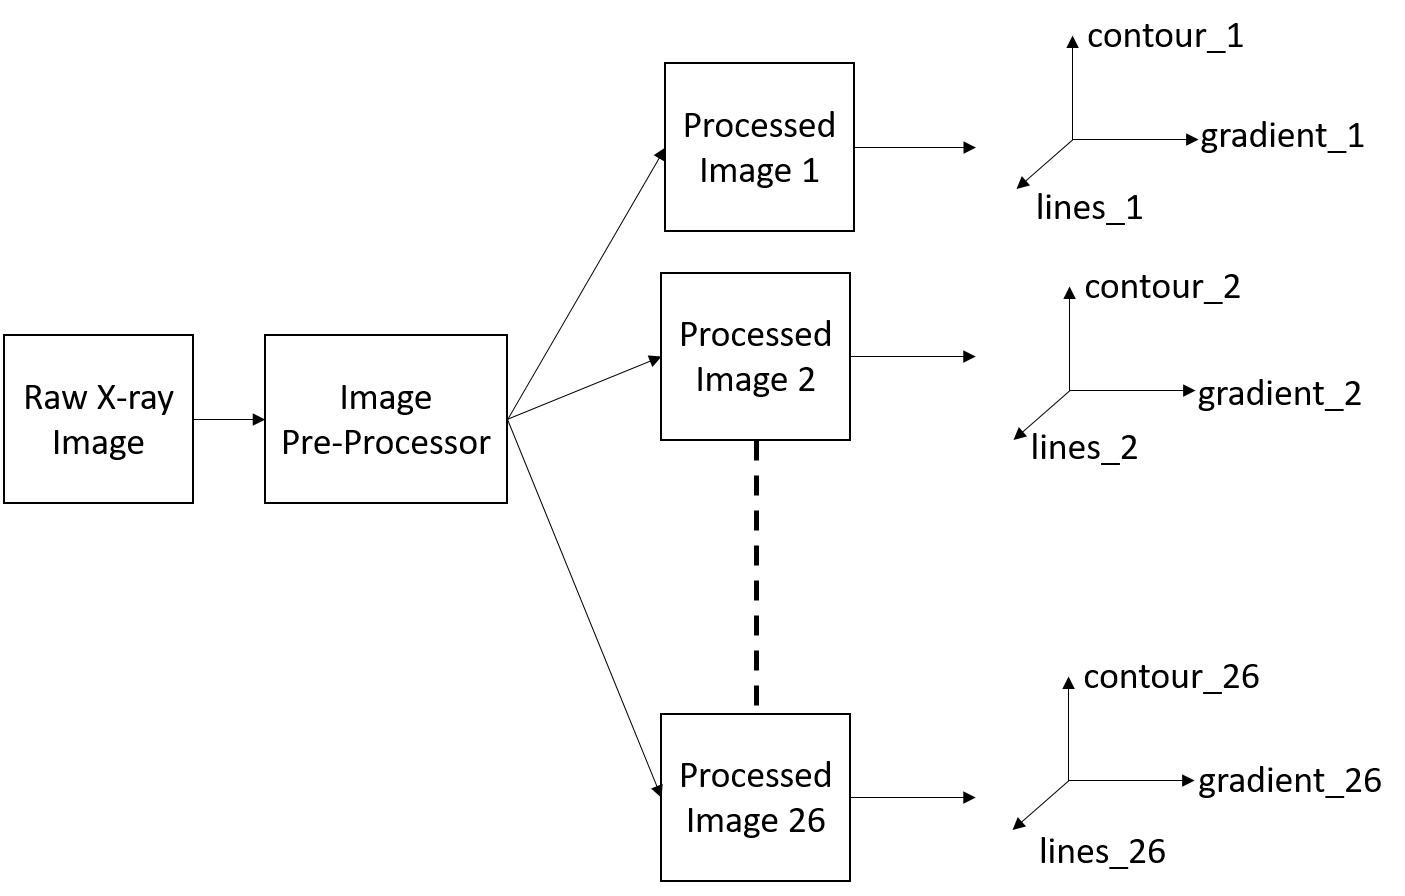
\includegraphics[scale=0.23]{image_processing.png}
		\caption{Data structure for all 26 pre-processed images to represent the original image}
		\label{fig: data_structure}
	\end{figure}
	
	\subsection{Dimensionality Reduction}
	\subsubsection{Principal Component Analysis}
	The first step is to determine the covariance matrix for original x-ray data. The covariance matrix is then used to determine the principal components. The number of principal components is proportional to the number of variables, $n$ within that dataset. The resultant principal components, $P_n$ are computed by determining the eigenvalues of the covariance matrix. The covariance matrix is in a symmetrical form. The eigenvalues found in the covariance matrix are the variances of the principal components. Since the number of principal component are proportional to the number of variables within an image, this means that there are $n$ eigenvalues. All eigenvalues, $\lambda$ are greater than or equal to zero. The largest eigenvalue corresponds to the first principal component. This applies to the next eigenvalue, until the i-th principal component. Therefore $\lambda_i$ corresponds to the i-th eigenvector.
	
	\begin{itemize}
		\item Step 1: The first step is to determine the covariance matrix for each original x-ray image, which has a three dimensional structure. Let the three dimensions be represented by $x$, $y$ and $z$. Thus the covariance matrix, $C$ can be expressed in \eqref{eq: covariance matrix}.
		\begin{equation}
		\label{eq: covariance matrix}
		C = 
		\begin{bmatrix}
		cov(x,x) & cov(x,y) & cov(x,z) \\
		cov(y,x) & cov(y,y) & cov(y,z) \\
		cov(z,x) & cov(z,y) & cov(z,z) \\
		\end{bmatrix}
		\end{equation}
		
		The result of $cov(x,x)$, $cov(y,y)$ and $cov(z,z)$ are eigenvalues of matrix $C$ which are the variances of the principal component.\\
		\item Step 2: The eigenvectors $v_1, v_2, v_3, ... , v_i$ corresponding to the eigenvalues $\lambda_1, \lambda_2, \lambda_3, ... , \lambda_i$ are calculated. Assuming that the eigenvalues are in descending order such that: $\lambda_1 \geq \lambda_2 \geq \lambda_3, \geq, ...,\geq \lambda_i$, then $\lambda_1$ is the first principal component and $v_1$ consists of the main characteristics for the given data. \\
		\item Step 3: The principal components that expresses the 26 images can be expressed as follows:
		\begin{equation}
		P_i = \lambda_{i1}Z_1 + \lambda_{i2}Z_2 + ... + \lambda_{in}Z_n
		\end{equation} 
		where $Z_n$ represents the 26 various images of the original x-ray image. \\
		\item Step 4: The low-dimension matrix is constructed by selecting the principal components that consists of the most variations of the data. Therefore the result mapping covariance matrix can be expressed as follows: 
		\begin{equation}
		M = [\lambda v_1, \lambda v_2, ... , \lambda v_n]
		\end{equation} \\
		\item Step 5: The low-dimension matrix is then constructed as follows:
		\begin{equation}
		Y = M^T \times \text{Original Data}
		\end{equation}
	\end{itemize}
	
	\subsubsection{Kernel Principal Component Analysis}
	Kernel Principal Component Analysis (KPCA) is centred around \eqref{eq: KPCA centred equation} \cite{Ibrahim_Baharudin2016}.
	\begin{equation}
		\label{eq: KPCA centred equation}
		\frac{1}{N}\sum_{i=1}^{N}\phi(x_i)=0
	\end{equation}
	\begin{itemize}
		\item Step 1: The covariance matrix is determined by \eqref{eq: KPCA covariance}, in which it produces a $M \times M$ matrix, where $M$ is the size of the dimensionality.
		\begin{equation}
			\label{eq: KPCA covariance}
			C = \frac{1}{N}\sum_{i=1}^{N}\phi(x_i)\phi(x_i)^T
		\end{equation} \\
		\item Step 2: The eigenvalues, $\lambda_k$ and eigenvectors, $V_k$ are determined using \eqref{eq: KPCA eigenvalues eigenvectors}, in which it can be re-written as \eqref{eq: KPCA eigenvalues eigenvector rewritten}.
		\begin{equation}
			\label{eq: KPCA eigenvalues eigenvectors}
			\frac{1}{N}\sum_{i=1}^{N}\phi(x_i)\left\{\phi(x_i)^TV_k\right\} = \lambda_k V_k
		\end{equation} 
		\begin{equation}
			\label{eq: KPCA eigenvalues eigenvector rewritten}
			V_k = \sum_{i=1}^{N}a_{aki}\phi(x_i)
		\end{equation} \\
		\item Step 3: \eqref{eq: KPCA substitution} is the result of substituting $V_kin$ from \eqref{eq: KPCA eigenvalues eigenvectors} into \eqref{eq: KPCA eigenvalues eigenvector rewritten}.
		\begin{equation}
			\label{eq: KPCA substitution}
			\frac{1}{N}\sum_{i=1}^{N}\phi(x_i)\phi(x_i)^T \sum_{j=1}^{N}a_{kj}\phi(x_j) = \lambda_{k}\sum_{j=1}^{N}a_{ki}\phi(x_i)
		\end{equation} \\
		\item Step 4: A kernel function is defined. Let the kernel function be defined by \eqref{eq: KPCA kernel function}.
		\begin{equation}
			\label{eq: KPCA kernel function}
			k(x_i, x_j) = \phi(x_i)^T\phi(x_j)
		\end{equation}\\
		\item Step 5: \eqref{eq: KPCA multiplied} is obtained by multiplying $\phi(x_l)^T$ to both sides of \eqref{eq: KPCA substitution}
	\end{itemize}
	\begin{equation}
	\label{eq: KPCA multiplied}
	\frac{1}{N}\sum_{i=1}^{N}(x_l, x_i)\sum_{j=1}^{N}a_{kj}k(x_i, x_j) = \lambda_k\sum_{i=1}^{N}a_{ki}k(x_l, x_i)
	\end{equation}
	\begin{itemize}
		\item Step 6:The notion matrix is expressed in \eqref{eq: KPCA notion matrix}.
		\begin{equation}
			\label{eq: KPCA notion matrix}
			K^2a_k = \lambda N K_{a_k} 
		\end{equation}
		where 
		\begin{equation}
			K_{i,j} = k(x_i, x_j)
		\end{equation}
		and $a_k$ is the Nth-dimensional vector of $a_{aki}$
		\begin{equation}
			a_{K} = [a_{ak1}a_{ake} . . . akN]^T
		\end{equation}
		in which $a_k$ can be solved using the following:
		\begin{equation}
			\label{eq: KPCA Kak}
			Ka_k = \lambda N a_k
		\end{equation} 
		\item Step 7: $\phi(x_i)$ does not always have zero-mean in the original space and it cannot be guaranteed that it is centred in the altered space. Therefore it can be used to created the Gram Matrix, $K'$ which can substitute the kernel matrix, $K$. The Gram matrix ensures that $\phi(x_i)$ is centred in the altered space. The Gram matrix is given by \eqref{eq: KPCA Gram Matrix} \cite{Ibrahim_Baharudin2016} \cite{Scholkopf2012}.
		\begin{equation}
			\label{eq: KPCA Gram Matrix}
			K' = K - 1_N K - 1K1_N + 1_NK1_N
		\end{equation}
		where $1_N = N \times N$ matrix in which all elements of the matrix is equal to $\frac{1}{N}$.\\
		\item Step 8: Dimensionality reduction is performed by constructing the kernel matrix from $K$ in \eqref{eq: KPCA notion matrix}. \\
		\item Step 9: The Gram Matrix is computed using \eqref{eq: KPCA Gram Matrix}. \\
		\item Step 10: \eqref{eq: KPCA Kak} is used to computed the Kernel principal components.
	\end{itemize}

	\subsubsection{Maximum Variance Unfolding}
	The MVU technique compresses the data by preserving the distances and the angles between the data points \cite{Shao2009}. 
	\begin{itemize}
		\item Step 1: Determine the smallest $k$ integer to construct the k-nearest graph that generates connected training samples, $\textbf{x}_1, . . . ,\textbf{x}_n$ \\
		\item Step 2: Using training samples, construct an $N \times N$ binary adjacency graph \textbf{S}. \\
		\item Step 3: \eqref{eq: MVU S setting} determines the values of $\textbf{S}_{ij}$.
		\begin{equation}
			\label{eq: MVU S setting}
			\textbf{S}_{ij} = 
			\begin{cases}
				1 & \text{if } \textbf{x}_i \text{ is k-nearest neighbour} \\
				0 & \text{otherwise}
			\end{cases}
		\end{equation}
		\item Step 3: Training the kernel matrix, $K$ by solving \eqref{eq: MVU kernel matrix}.
		\newline
		Maximize trace(\textbf{K}) subject to:
		\begin{equation}
			\label{eq: MVU kernel matrix}
			\begin{cases}
				(1) &\textbf{K} \geq 0 \\
				(2) &\sum_{ij}\textbf{k}_{ij} = 0 \\
				(3) &\textbf{K}_{ii} - \textbf{2K}_{ij} + \textbf{K}_{jj} = ||\textbf{x}_i - \textbf{x}_j||^2
			\end{cases}
		\end{equation}
		\item Step 4: Eigen-decomposition for $\textbf{K}$ is performed and the reduce dimension is set to the intrinsic dimension, $d$ which is determined by the eigenvalues of $\textbf{K}$.\\
		\item Step 5: The d-dimensional MVU is computed, which embeds the training samples, $\textbf{y}_1, . . . , \textbf{y}_N$. The training samples can re-written and it is expressed in \eqref{eq: MVU training samples}.
		\begin{equation}
			\label{eq: MVU training samples}
			\textbf{y}_i = [\sqrt{\lambda_1}\alpha_1^1, . . . ,\sqrt{\lambda_d}\alpha_i^d]^T
		\end{equation}
		\item Step 6: A basis linear vector projection is trained such that it approximates the mapping between the input vector, $\text{x}_i$ to the output vector, $\textbf{y}_i$ by linear regression.
	\end{itemize}
	
	\subsection{Neural Network}
	An artificial neural network consists of three different layers: input layer, hidden layer and output layer. There are weighted connections which link the three layers together. The chosen neural network consists of one hidden layer for simplicity purposes. 
	A graphical layout of the neural network is shown in Figure \ref{fig: neural_network}.
	\begin{figure}[!h]
		\centering
		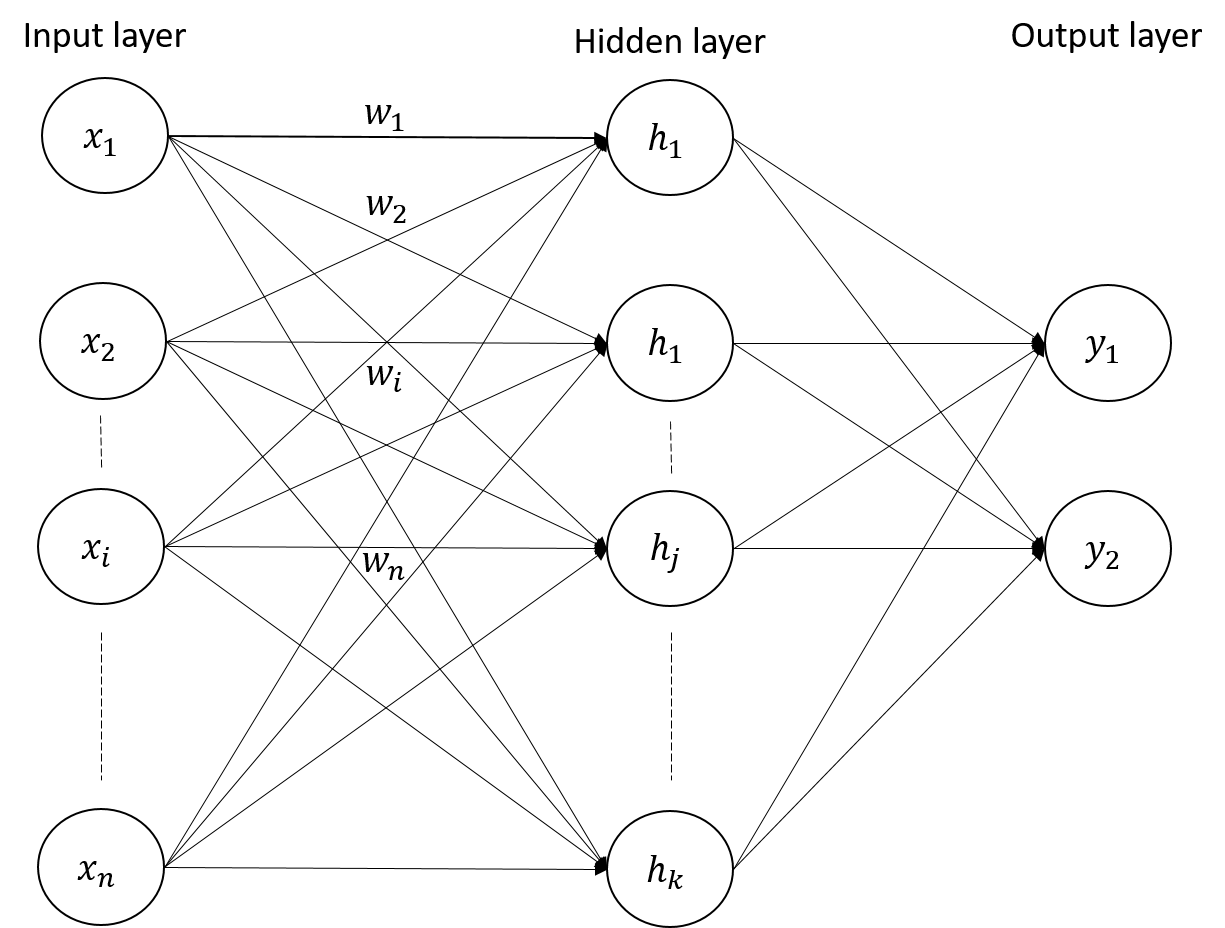
\includegraphics[scale=0.25]{neural_network.png}
		\caption{Neural Network Layout showing the input, hidden and output layers}
		\label{fig: neural_network}
	\end{figure}
	
	The weights are factors which assist with the automated decision making process. The weights values are determined through a training process. The chosen neural network training method is back-propagation. The training process makes use of the resultant matrices from the dimensionality reduction technique. The operations for training the neural network is described below:
	
	\subsubsection{Step 1:} 
	The first step is to initialize the weights in which each weight can be randomly assigned a value (representing the weight), since it will be corrected at a later stage.
	
	\subsubsection{Step 2:}
	The inputs and the desired outputs are defined. The inputs are the matrices obtained from the dimensionality reduction technique, whilst the outputs are the desired outcome result for corresponding input matrices.
	
	\subsubsection{Step 3:}
	The net input into each node, $net_{h_k}$ in the hidden layer is computed as follows for $i = \left\{1, 2, ..., n\right\}$ and $k = \left\{1, 2, ..., k\right\}$:
	\begin{equation}
		net_{h_k} = \sum_{i = 0}^{n} w_{ik}x_i 
	\end{equation}
	
	\subsubsection{Step 4:}
	The output for each node in the hidden layer is calculated by applying the logistic function. The calculation for the first node, $h_1$ is performed as follows:
	\begin{equation}
		Out_{h_k} = \frac{1}{1 + e^{-net_{h_k}}}
	\end{equation}
	
	\subsubsection{Step 5:}
	The net input and output for the nodes at the output layer is computed in the same manner as shown in Step 3 and 4, which given as for $j = \left\{1, 2, ..., k\right\}$ and $m = \left\{1, 2\right\}$:
	\begin{equation}
		net_{y_m} = \sum_{j = 0}^{k} w_{jm}h_j
	\end{equation}
	\begin{equation}
		Out_{y_m} = \frac{1}{1 + e^{-net_{y_m}}}
	\end{equation}
	The output of the nodes, $Out_{y_m}$ are crucial for the next step. 
	
	\subsubsection{Step 6:}
	The objective of back-propagation is to update each weight within the network such that the computed output is as close to the target as possible. This is done by first calculating the total error between the actual output and the target. The total error is computed as follows:
	\begin{equation}
		E_{total} = \sum \frac{1}{2} (target - output)^2
	\end{equation}
	
	\subsubsection{Step 7:}
	The total error is used to adjust the weights within the neural network. This adjustment is performed over $t$ iterations such that the total error is at its minimal. The error minimal value can be a predefined threshold value. The adjustments of the weights are expressed as follows:
	\begin{equation}
		w_{im}(t) = w_{im}(t-1)+\eta\delta_i(t)y_m(t)
	\end{equation}
	where:
	\begin{align*}
		& \delta_i(t) = 
		\begin{cases}
			y_m(t)(1 - y_m(t))\times e_m(t) & m \text{ } \epsilon \text{ output layer}\\
			y_m(t)(1 - y_m(t)) & \text{if not}
		\end{cases} \\
		& 0 < \eta < 1 \\
		& \eta = \text{learning rate} \\
		& e_m(t) = \text{error at node m for t iteration}
	\end{align*}
	
	\subsection{Further Investigations}
	Further investigations can be conducted to extend the two-step system to detect the presence of Tuberculosis disease (TB) as well as into the manufacturing field to detect fractures within manufactured products or even gaps (air bubbles) in welded components. However, this will require additional data and may need further image pre-processing. 
	
	\section{Time Management and Milestones}
	\label{sc: Time Management and Milestones}
	Table \ref{time_management} and Table \ref{tb: image table} illustrate the tasks that need to completed in order to obtain the results for the research.
	\begin{table}[!h]
		\centering
		\caption{Table showing the time management for conducting the proposed research.}
		\label{time_management}
		\begin{tabular}{| c | p{2.5cm} | p{4.5cm} |}
			\hline
			& Period & Task Description \\
			\hline \hline
			1 & Jan 11 - Apr 10 2017 & Work on Research Proposal for submission\\
			\hline
			2 & Apr 11 - Jul 10 2017 & Develop system for image enhancement and feature extraction for x-ray images \\
			\hline
			3 & Jul 11 - Oct 10 2017 &  Develop the system for dimensionality reduction. This includes testing the system\\
			\hline
			4 & Oct 11 - Jan 10 2018 & Develop neural network along with training algorithm for the detection of bone fracture \\
			\hline
			5 & Jan 11 - Apr 10 2018 & Work on first letter paper \\
			\hline
			6 & Apr 11 - Jul 10 2018 & Integration of both dimensionality reduction module and the neural network module \\
			\hline
			7 & Jul 11 - Oct 10 2018 & Work on second letter paper\\
			\hline
			8 & Oct 11 - Jan 10 2019 & Work on Dissertation \\
			\hline
		\end{tabular}
	\end{table}
	
	\begin{table}[!h]
		\centering
		\caption{Table showing the milestones that need to be achieved for the research}
		\label{tb: milestones}
		\begin{tabular}{| c | l | p{5cm} |}
			\hline 
			& Date & Task \\
			\hline \hline
			1 & Apr 10 2017 & Submit research proposal for approval\\
			\hline
			2 & Jul 10 2017 & Complete development of image enhancement and feature extraction system \\
			\hline
			3 & Oct 10 2017 & Complete development of the dimensionality reduction model \\
			\hline
			4 & Jan 10 2018 & Complete development of neural network model \\
			\hline
			5 & Apr 10 & Submit first letter paper \\
			\hline
			6 & Jul 10 2018 & All models fully integrated \\
			\hline
			7 & Aug 10 2018 & All results for research is obtained \\
			\hline
			8 & Oct 10 2018 & Submit second letter paper \\
			\hline
			9 & Jan 10 2019 & Submit dissertation for approval \\
			\hline
		\end{tabular}
	\end{table}

	\section{Conclusion}
	\label{sc: Conclusion}
	The research proposed in this paper is to determine an optimal dimensionality reduction technique for a two-step system to detect the presence of a bone fracture from an x-ray image. The dimensionality techniques mentioned in the proposed methodology are PCA, KPCA and MVU. The dimensionality reduction technique is implemented in the first step of the system, whilst the second step is a neural network component. The neural network component is trained using back-propagation. The data structure is based on the image pre-processing technique, in which the data structure is constructed from the 26 resultant images as well as the three extracted features, gradient, lines and contours. The optimal dimensionality reduction technique is determined by the performance of each technique. The performance is based on detection accuracy, error rate and execution speed. Additionally, further investigations will be conducted to extend the system to the detection of Tuberculosis disease (TB) as well as the manufacturing field to detect fractures within axle components.
	
	%\bibliographystyle{witseie}
	\bibliographystyle{IEEEtran}
	\bibliography{standard_2}
	
\end{document}